\documentclass[preprint]{sigplanconf}

\usepackage{amsmath,amssymb,amsopn,amsthm}
\usepackage[T1]{fontenc}
\usepackage{algorithmic,algorithm}
\usepackage{multirow}
\usepackage{cleveref}
\usepackage{graphicx}
\usepackage[usenames,dvipsnames]{xcolor}
\usepackage{verbatim}
\usepackage{stfloats}

\usepackage{tikz}
\usetikzlibrary{fit}
\usepackage{pgfplots}
\usepackage{pgfplotstable}
\pgfplotsset{compat=1.12}

\newcommand\todo[1]{{\color{NavyBlue} \footnote{\color{NavyBlue} TODO: {#1}}}}
\newcommand\citneeded[1]{{\color{NavyBlue} \cite{?}\footnote{\color{NavyBlue} citation needed. #1}}}

\newcommand\newterm[1]{{\it #1}}
\newcommand\R{\mathbb{R}}
\newcommand\N{\mathbb{N}}
\newcommand\B{\mathbb{B}}
\newcommand\T{\mathcal{T}}
\renewcommand\S{\mathcal{S}}

\newcommand\lspan[2]{\multicolumn{#1}{@{}l}{#2}}
\newcommand\cspan[2]{\multicolumn{#1}{@{}c}{#2}}

\makeatletter
\newcommand{\LeftEqNo}{\let\veqno\@@leqno}
\makeatother

\newcommand\limplies{\rightarrow}
\newcommand\liff{\leftrightarrow}

% author comment macros
\newcommand\authornote[3]{{\color{#2} \footnote{\color{#2} {#1}: {#3}}}}

\newcommand\asolar[1]{\authornote{AS}{BrickRed}{#1}}  % Armando
\newcommand\cel[1]{\authornote{CL}{OliveGreen}{#1}}   % Charles
\newcommand\rch[1]{\authornote{RC}{RoyalPurple}{#1}}  % Rezaul
\newcommand\pga[1]{\authornote{PG}{RawSienna}{#1}}    % Pramod
\newcommand\coa[1]{\authornote{SI}{NavyBlue}{#1}}     % Shachar

\include{macros}

\begin{document}


\special{papersize=8.5in,11in}
\setlength{\pdfpageheight}{\paperheight}
\setlength{\pdfpagewidth}{\paperwidth}

%\conferenceinfo{CONF 'yy}{Month d--d, 20yy, City, ST, Country} 
%\copyrightyear{20yy} 
%\copyrightdata{978-1-nnnn-nnnn-n/yy/mm} 
%\doi{nnnnnnn.nnnnnnn}

%\titlebanner{banner above paper title}        % These are ignored unless
%\preprintfooter{short description of paper}   % 'preprint' option specified.

%\title{Bellmania: Deriving Implementations from Specifications by Transformation}
%\title{Solver-Aided Transformational Synthesis of Divide-and-Conquer Dynamic Programming Algorithms}
\title{Deriving Divide-and-Conquer Dynamic Programming Algorithms Using 
  Solver-Aided Transformations}

%\authorinfo{Shachar Itzhaky}
%           {MIT CSAIL}
%           {shachari@mit.edu}
\authorinfo{Double-blind submission}
           {}
           {}

\maketitle

\begin{abstract}
Programmers almost never write optimal code on the first phase.
Instead, they usually begin with a simplified, possibly inefficient, or even
na\"ive implementation. When the result is satisfactory, they would move
on to revise the code in order to improve performance. These normally
change the code considerably compared to the original version. It is especially
true for code that targets multi-core processors, since many considerations
must be taken into account for parallel code in order to utilize all available
cores.

Clearly, each iteration becomes more tedious as the code increases in complexity,
and naturally holds more chance of introducing defects. The programmer must
exercise care to make sure that each version is functionally equivalent to the
previous one. This is when mechanical reasoning can prove useful, by 
(a) packaging familiar techniques as routines, thus avoiding repetitive work, and
(b) checking each modification step, warning the developer when functionality
may be accidentally changed.

We present Bellmania, a framework comprising of a language for specifying
dynamic programming algorithms as recurrences,
and a calculus that facilitates gradual transformation of these 
specifications into efficient implementations.
In particular, it supports using the Divide and Conquer technique to derive
parallel implementations that optimally utilize memory caches.
\end{abstract}

\category{CR-number}{subcategory}{third-level}

\keywords
synthesis, dynamic programming, smt

\section{Introduction}
\label{intro}


\newcommand{\xidx}{i}
\newcommand{\yidx}{j}
\newcommand{\xw}[1]{w_{#1}}
\newcommand{\yw}[1]{w'_{#1}}

Software synthesis techniques can be broadly classified into two categories: \emph{inductive} approaches which generalize from concrete values or execution traces, and \emph{deductive} approaches which derive an implementation from a specification through deductive reasoning steps. Inductive synthesis techniques have been the focus of significant renewed interest thanks to two important developments: (a) the discovery of techniques that leverage SAT/SMT solvers to symbolically represent and search very large spaces of possible programs~\cite{APLAS09/Solar-Lezama, PLDI11/Gulwani, Onward13/Torlak}, and (b) the use of counterexample-guided inductive synthesis (CEGIS), which allows one to leverage inductive techniques to find programs that satisfy more general specifications as long as one has access to an oracle that can check whether a given candidate solution satisfies the specification~\cite{APLAS09/Solar-Lezama}. Deductive techniques, however, still hold some important advantages over inductive approaches; in particular, their scalability is not limited by the power of a checking oracle, because the correctness of the implementation is guaranteed by construction; this makes them better suited for synthesizing large programs with strong correctness guarantees. 

In this paper, we present a new approach to deductive synthesis based on \emph{solver-aided tactics} that preserves the benefits of deductive synthesis techniques but reduces the burden on the user by relying heavily on the ability of SMT solvers to reason about the validity of transformations and lift the level of abstraction of deductive transformation rules. 
We believe the approach has the potential to be generally applicable to a variety of synthesis problems, but in this paper, we focus on a particular domain of \emph{divide-and-conquer dynamic programming} algorithms, and the Bellmania system that was constructed to address its special features. As we illustrate in the next section, this domain is challenging not just as a synthesis target, but also for human experts. Therefore, in addition to serving as a test bed for a new synthesis approach, the development of Bellmania is a significant achievement in itself.

Our work on solver-aided tactics builds on prior work on the StreamBit project~\cite{PLDI05/Solar-Lezama}, which introduced the idea of transformation rules with missing details that can be inferred by a symbolic search procedure, as well as the pioneering work on the Leon synthesizer, which has explored the use of deductive techniques to improve the scalability of inductive synthesis. However, our approach is unique the way it leverages the SMT solver in the context of deductive synthesis: (a) the solver can directly check that a program term is equivalent to another term, thus merging branches and reducing repetitive manual labor, (b) The solver can prove validity of side conditions that ensure the soundness of each individual transformations. The tactics in our library gain more freedom and can be designed to be much more generic than if they were purely symbolic, since they do not have to represent logically valid equivalences: instead, they can represent equalities that are {\bf sometimes} true, and carefully check each context in which they are applied. 

Overall, we make the following contributions.
\begin{itemize}
\item We introduce \emph{solver-aided tactics} as a way to raise the level of abstraction of deductive synthesis.
\item We develop a small set of formal \newterm{solver-aided tactics} that can be used to transform a class of recurrence
  specifications, written in a simple functional language, 
  into equivalent divide-and-conquer programs, that admit parallel cache-local
  implementations, in a principled, systematic manner.
\item We prove that these tactics are semantics-preserving, assuming some side conditions are met
  at the point when the tactic is applied.
  \item We show that the side conditions can be effectively translated into first-order closed
  formulas, and verified automatically by SMT solvers.
\item We demonstrates the first system capable of generating provably correct implementations of divide-and-conquer implementations from a high-level description of the algorithm. 
\end{itemize} 

\section{Divide-and-Conquer DP}
\label{divide}

Most readers are likely familiar with the Dynamic Programming (DP) technique of Richard Bellman~\cite{03/Bellman:DP} to construct an optimal solution to a problem by combining together optimal solutions to many overlapping sub-problems. The key to DP is to exploit the overlap in order to explore otherwise exponential-sized problem spaces in polynomial time. Dynamic programs are usually described through recurrence relations that specify how the cells in a DP table must be filled up using solutions already computed for other cells, but recent research has shown that it is possible to achieve order-of-magnitude performance improvements over this standard implementation approach by developing \emph{divide-and-conquer}  implementation strategies that recursively
partition the problem into smaller subproblems.  These strategies exhibit better temporal locality, and the partitioning can expose more
optimization opportunities (see, e.g., \cite{IPDPS15/Tithi}).  Even when compared with tiled implementations optimized by the best polyhedral compilers, 
the divide-and-conquer implementations still show significantly better performance, in some cases by more several orders of magnitude. For example, Tithi \etal{} have shown that for classical DP problems such as Floyd-Warshall, the parallel divide-and-conquer implementation is  8x faster  across a range of problem sizes compared with a parallel tiled implementation~\cite{IPDPS15/Tithi}. These performance differnces matter because  DP is central to many important domains ranging from logistics to computational biology; as an illustrative example, a recent textbook \cite{DurbinEdKr98} on biological sequence analysis lists 11 applications of DP in bioinformatics just in its introductory chapter with many more in chapters that follow.

% Decided to remove the figure. Don't want to give the impression that we are trying to get credit from results from another paper.
%\begin{figure*}[b]
% \centering
% \resizebox{.9\textwidth}{!}{\begin{tikzpicture}
	\begin{axis}[
	    title=Parenthesis,
	    ymode=log,
		xlabel=$n$,
		ylabel=Time ({\it s}),
		scaled x ticks=false, %{real:1000}
		log basis y=2, ymajorgrids=true]
	\addplot[color=blue!50!white,ultra thick,mark=*,smooth] table[x=n/Time(s),y=COZ] {data/plot1.dat}
	  [yshift=-8pt] node[pos=0] {CO};
	\addplot[color=red!70!white,ultra thick,mark=*,smooth] table[x=n/Time(s),y=Tiled/Par] {data/plot1.dat}
	  [yshift=-10pt] node[pos=0] {PluTo};
	\end{axis}
\end{tikzpicture}
\begin{tikzpicture}
	\begin{axis}[
	    title=Gap,
	    ymode=log,
		xlabel=$n$,
		scaled x ticks=false, %{real:1000}
		log basis y=2, ymajorgrids=true]
	\addplot[color=blue!50!white,ultra thick,mark=*,smooth] table[x=n/Time(s),y=COZ] {data/plot2.dat}
	  [yshift=-8pt] node[pos=0] {CO};
	\addplot[color=red!70!white,ultra thick,mark=*,smooth] table[x=n/Time(s),y=Tiled/Par] {data/plot2.dat}
	  [yshift=-8pt] node[pos=0] {PoCC};
	\end{axis}
\end{tikzpicture}
\begin{tikzpicture}
	\begin{axis}[
	    title=Floyd-Warshall,
	    ymode=log,
		xlabel=$n$,
		scaled x ticks=false, %{real:1000}
		log basis y=2, ymajorgrids=true]
	\addplot[color=blue!50!white,ultra thick,mark=*,smooth] table[x=n/Time(s),y=COZ] {data/plot3.dat}
	  [yshift=-8pt] node[pos=0] {CO};
	\addplot[color=red!70!white,ultra thick,mark=*,smooth] table[x=n/Time(s),y=Tiled/Par] {data/plot3.dat}
	  [yshift=-8pt] node[pos=0] {PoCC};
	\end{axis}
\end{tikzpicture}
}
% \caption{\label{intro:performance}
%  Comparison of the the best performance obtained using polyhedral compilers 
%  (PluTo\,\cite{HPC10/Pouchet}, PoCC\,\cite{PLDI08/Bondhugula})
% for parallelization, vs. manually crafted recursive divide-and-conquer implementations (CO),
%  taken from~\cite{IPDPS15/Tithi}.}
% \end{figure*}


Before diving into the details of how solver-aided tactics can be used to derive divide-and-conquer dynamic programming, it is important to explain how an algorithm's expert would go about deriving such an implementation by hand.
As a motivating example, we consider the Simplified Arbiter problem.
Two processes $x$ and $y$ are scheduled to run $|x|$ and $|y|$ time slots,
respectively. Execution starts at $t=0$, and the length of each time slot is
one time unit. The cost for scheduling the slots $[a..b)$ of $x$ at $t=a+c$
is given by $\xw{abc}$, and the cost for schedulting the slots $[a..b)$ of $y$
at same $t=a+c$ is given by $\yw{abc}$.

\begin{figure}[b]
\begin{tabular}{@{\hspace{-1pt}}r@{~}l@{}}
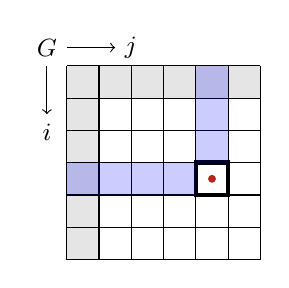
\begin{tikzpicture}[x=4.1mm,y=4.1mm,baseline=(center), remember picture]
  \coordinate(center) at (3,3);
  \draw[step=1] (0,0) grid (6,6);
  \draw[ultra thick] (4,2) rectangle +(1,1);
  %\node(Gij) at (4.5,2.5) {\tiny $\scriptscriptstyle\langle i,j\rangle$};
  \node[circle,fill=BrickRed,inner sep=0,minimum size=1mm](Gij) at (4.5,2.5) {};
  \fill[black,opacity=0.1] (0,5) rectangle (6,6);
  \fill[black,opacity=0.1] (0,0) rectangle (1,5);
  \fill[blue,opacity=0.2] (0,2) rectangle (4,3);
  \fill[blue,opacity=0.2] (4,3) rectangle (5,6);
  \node[anchor=south east](G) at (0,6) {\small$G$};
  \draw[->] (G.east) -- +(1.5,0) node[anchor=west] {\small $j$};
  \draw[->] (G.south) -- +(0,-1.5) node[anchor=north] {\small $i$};
\end{tikzpicture}
&
\small
$
\begin{array}{l@{}}
	\tikz[overlay, remember picture]{\draw[BrickRed] (0,0) -- (Gij);}
	G_{ij} ~=~ \\
	~
	\begin{cases}
		0                        & i=j=0 \\
		\yw{0j0}                  & i=0, j>0 \\
		\xw{0i0}                 & i>0, j=0 \\
		\begin{array}{@{}l@{\hspace{-1pt}}l@{\hspace{-4pt}}}
		  \min\langle & \underset{0\leq q<j}\min ~ G_{iq} + \yw{qji},  \\
		              & \underset{0\leq p<i}\min ~ G_{pj} + \xw{pij}~\rangle
		\end{array}              & i,j>0
	\end{cases}
\end{array}
$
\end{tabular}
\vspace{5pt}
\caption{Recurrence equation and cell-level dependencies.}
\label{intro:arbiter spec}
\end{figure}


The optimal cost for scheduling the first $i$ slots of $x$ and the first $j$ slots
of $y$ is given by the recurrence in \Cref{intro:arbiter spec}. When $i$ is zero, it means that
only $y$ has been scheduled, so the cost is $\yw{0j0}$, and similarly when $j$ is zero, 
the cost is $\xw{0i0}$. When $i$ and $j$ are both positive, there are two options:
either the schedule ends with an allocation to $x$, 
where slots $[p..i)$ of $x$ were scheduled at $t=p+j$, and the cost is 
$G_{pj} + \xw{pij}$; or it ends with an allocation to $y$, where
slots $[q..j)$ of $y$ were scheduled at $t=i+q$, and the cost is $G_{iq} + \yw{qji}$.
The minimum over all respective $p<i$ and $q<j$ is taken.
Eventually, the optimal cost of the entire schedule is given by $G_{|x||y|}$.

\begin{paragraph}{Iterative Algorithm.}
Using a standard dynamic programming method, Richard, an algorithms expert, computes this recurrence
with an iterative program by understanding the dependency pattern:
to compute the $\min\langle\rangle$ expression in \Cref{intro:arbiter spec} and find the optimal
values for $p$ and $q$, the algorithm needs information from all cells above and to the left of $G_{ij}$.
In particular, each value $G_{ij}$ is computed from other values $G_{i'j'}$ with lower
indexes, $i'<i$, ~$j'<j$. 
Therefore, considering $G$ as a two-dimensional array, it can be filled in a single pass from left to right and from top
to bottom.
\end{paragraph}

\newcommand\FORLINE[1]{\STATE\algorithmicfor~{#1} \algorithmicdo~}

\begin{algorithm}
\renewcommand\arraystretch{1.3}
\begin{algorithmic}
  \STATE $G_{00} := 0$
  \FORLINE{$j=1..|y|$}  $G_{0j} := \yw{0j0}$  
  \FOR{$i=1..|x|$}
    \STATE $G_{i0} := \xw{0i0}$
    \FOR{$j=1..|y|$}
      \STATE $G_{ij} :=
        \begin{array}[t]{@{}l@{~}l} 
          \min\langle & \underset{0\leq q<j}\min ~ G_{iq} + \yw{qji}, \underset{0\leq p<i}\min ~ G_{pj} + \xw{pij}~\rangle \\         
        \end{array}$
    \ENDFOR
  \ENDFOR
\end{algorithmic}
\caption{\label{intro:iterative}
   Iterative Simplified Arbiter}
\end{algorithm}


\newcommand\qbox[1]{\fbox{\scriptsize#1}}

\begin{paragraph}{Divide-and-Conquer Algorithm.}

\begin{figure}
\centering
\begin{tabular}{c@{\hspace{.5in}}c}
$
\renewcommand\arraystretch{2}
\begin{array}[b]{c|c|c|c|}
  \multicolumn{2}{c}{} & \multicolumn{2}{c}{J} \\ \cline{3-4}
  \multicolumn{2}{c}{} & \multicolumn{1}{c}{J_0}  & \multicolumn{1}{c}{J_1}\\ \cline{3-4}
  \multirow{2}{*}{$I$} & I_0 & 1 & 2 \\ \cline{3-4}
    & I_1 & 3 & 4 \\ \cline{3-4}
\end{array}
$
& 
$\begin{array}[b]{l}\qbox1 \rightsquigarrow \qbox2 \\ 
\qbox1 \rightsquigarrow \qbox3 \\ \qbox2\rightsquigarrow \qbox4 \\ \qbox3 \rightsquigarrow \qbox4\end{array}$
\end{tabular}
\vspace{5pt}
\caption{\label{intro:quadrants}
  Dividing a two-dimensional array into quadrants; the dependencies are shown on the right.}
\end{figure}

Divide-and-conquer is an algorithm development pattern (\cite{SODA06/Chowdhury}, \cite{SPAA08/Chowdhury})\coa{should these (SODA/SPAA) be the ones to cite here?}, 
where the DP table is partitioned into regions, and each region is expressed as a sub-problem
to be solved.

In our case, Richard takes the two-dimensional array $G$ and partitions it into
quadrants, as illustrated in \Cref{intro:quadrants}. He then applies the same reasoning
as in the iterative case, concluding that the computations of 2 and 3 depend on 1,
and the computation of 4 depends on 2 and 3.
\end{paragraph}

Richard \emph{stratified} the computations on these quadrants into the following
four steps:
\begin{algorithmic}[1]
  \STATE Compute \qbox1 (using only input data $w,w'$).
  \STATE Compute \qbox2 using data from \qbox1.
  \STATE Compute \qbox3 using data from \qbox1.
  \STATE Compute \qbox4 using data from \qbox2 and \qbox3.
\end{algorithmic}

Each step depends only on a subset of the steps that came before it, 
as illustrated by \Cref{intro:chain}. However, this is not yet a divide-and-conquer algorithm: 
of the four steps, only step \qbox1{} is an instance of the original problem; all the other steps
look somewhat different from the original problem and lack significant locality. With some algebraic manipulation, however, 
it is possible to define each of the four steps above recursively, leading to a true divide-and-conquer algorithm with very high locality 
and significantly improved performance relative to the iterative algorithm.

To illustrate how this is done, we first introduce a small amount of notation. 
We define $I$ and $J$ to be the index sets for the rows and columns, respectively.
We then define partitions $I=I_0\cup I_1$ and $J=J_0\cup J_1$ as in \Cref{intro:quadrants}.
$G$ is now parameterized on those index sets;

\begin{equation}
\begin{array}{l@{}l}
	G^{^{IJ}}_{(i:I)\,(j:J)} ~=~  \\
	\qquad
	\begin{cases}
		0                         & i=j=0 \\
		w_{0j0}                   & i=0, j>0 \\
		w'_{0i0}                  & i>0, j=0 \\
		\begin{array}{@{}l@{~}l}
		  \min\langle & \underset{q\in J\cap[0,j)}\min ~ G^{^{IJ}}_{iq} + \yw{qji}, \\
		              & \underset{p\in I\cap[0,i)}\min ~ G^{^{IJ}}_{pj} + \xw{pij}~\rangle
		\end{array}              & i,j>0
	\end{cases}
\end{array}
\end{equation}

The computation of \qbox1 corresponds to computing $G^{IJ}$ within the sub-domain 
$I_0\times J_0$, making it an exact copy of $G^{I_0J_0}$. This is due to the fact
that for $j\in J_0$, ~$J\cap[0,j)=J_0\cap[0,j)$, and for $i\in I_0$, ~$I\cap[0,i)=I_0\cap[0,i)$.

On the other hand, the computation of \qbox2 is {\bf not} a mere copy of $G^{I_0J_1}$, 
because the range $q\in J\cap[0,j)$ is not a subset of $J_1$, so that
some of the recursive references $G_{iq}$ are outside of \qbox2.

This can be addressed by splitting that range, adding yet range another parameter to $G$.

\begin{equation}\LeftEqNo
\begin{array}{l@{}l}
	G^{^{IJJ'}}_{(i:I)\,(j:J)} ~=~  \\
	\qquad
	\begin{cases}
		0                         & i=j=0 \\
		w_{0j0}                   & i=0, j>0 \\
		w'_{0i0}                  & i>0, j=0 \\
		\begin{array}{@{}l@{~}l}
		  \min\langle & \underset{~q\in J'~}\min ~ G^{^{IJ'\!J'}}_{iq} + \yw{qji}, \\
		              & \underset{q\in J'\cap[0,j)}\min ~ G^{^{IJJ}}_{iq} + \yw{qji}, \\
		              & \underset{p\in I\cap[0,i)}\min ~ G^{^{IJJ'}}_{pj} + \xw{pij}~\rangle
		\end{array}              & i,j>0
	\end{cases}
\end{array}
\end{equation}

The computation of \qbox2 is now a copy of $G^{I_0J_1J_0}$. ~$G$ can be further generalized in the following
way:

\newcommand{\Ggen}{H}

\begin{equation}\LeftEqNo
\begin{array}{l@{}l}
	\Ggen^{^{IJ}}_{(i:I)\,(j:J)\,\psi} ~=~  \\
	\qquad
	\begin{cases}
		0                         & i=j=0 \\
		w_{0j0}                   & i=0, j>0 \\
		w'_{0i0}                  & i>0, j=0 \\
		\begin{array}{@{}l@{~}l}
		  \min\langle & \psi_{ij}, \\
		              & \!\underset{q\in J\cap[0,j)}\min ~ G^{^{IJJ}}_{iq} + \yw{qji}, \\
		              & \!\underset{p\in I\cap[0,i)}\min ~ G^{^{IJJ}}_{pj} + \xw{pij}~\rangle
		\end{array}              & i,j>0
	\end{cases}
\end{array}
\label{intro:Ggen}
\end{equation}

It is easy to see that both $G$ and \qbox1 can be expressed in terms of $\Ggen^{IJ}$ by making $\psi_{ij}=\infty$, 
but more importantly, \qbox2 can now also be expressed in terms of $\Ggen^{I_0J_1}$ by making 
$\psi_{ij} =  \underset{q\in J_0}\min ~ G^{I_0J_0J_0}_{iq} + \yw{qji}$.
Moreover, the calls to $G$ inside $\Ggen$ can be replaced with recursive calls to $\Ggen$ itself,
giving the form: 

\begin{equation}\LeftEqNo
\begin{array}{l@{}l}
	\Ggen^{^{IJ}}_{(i:I)\,(j:J)\,\psi} ~=~  \\
	\qquad
	\begin{cases}
		0                         & i=j=0 \\
		w_{0j0}                   & i=0, j>0 \\
		w'_{0i0}                  & i>0, j=0 \\
		\begin{array}{@{}l@{~}l}
		  \min\langle & \psi_{ij}, \\
		              & \!\underset{q\in J\cap[0,j)}\min ~ H^{^{IJ}}_{iq} + \yw{qji}, \\
		              & \!\underset{p\in I\cap[0,i)}\min ~ H^{^{IJ}}_{pj} + \xw{pij}~\rangle
		\end{array}              & i,j>0
	\end{cases}
\end{array}
\end{equation}

The same approach can be used to develop the computations of \qbox3 and \qbox4.
The sub-computation of $\psi$ can also be transformed into four recursive sub-computations, further improving the locality of the resulting algorithm.
So through these kind of transformations, it is possible to break the computation of the original $G$ into four (or more) subcomputations, each of which can be itself recursively partitioned into four subcomputations, giving us a true divide-and-conquer algorithm.
When the pieces become small enough, the iterative algorithm (\Cref{intro:iterative}) is executed.

\medskip
As was outlined in \Cref{divide}, prior work has shown that the performance results that can be achieved through these transformations can be dramatic. Unfortunately, the line of reasoning that was followed in this section can get quite complicated for most dynamic programming algorithms, and producing a correct divide-and-conquer algorithm for a given dynamic programming problem is considered quite difficult even by the researchers who originally pioneered this technique. 

In the following sections, we describe the parts that make Bellmania --- a formal framework for deriving algorithms from specifications. 
It utilizes \newterm{solver-aided tactics} to generate provably correct pseudo-code; 
this approach is demonstrated by engineering specialized tactics for the domain of divide-and-conquer DP.


\begin{figure}
\centering
\begin{tikzpicture}[>=latex,x=6mm,y=6mm,
    every path/.style={step=1},
    every node/.style={inner sep=.5pt},
    block/.style={rectangle,draw,thick,fill=Orange, fill opacity=0.15, inner sep=0}]
    
  \def\dx{1.75cm}
  \def\w{3mm}
    
  \draw (0,0) grid (2,2);
  %\node(1) at (.5,1.5) {1};   \node(2) at (1.5,1.5) {2};
  %\node(3) at (.5,.5) {3};    \node(4) at (1.5,.5) {4};

  \node[inner sep=0] at (2.5,1) {\includegraphics[width=\w]{img/arrow}};

  \tikzset{xshift=\dx}
  
  \draw (0,0) grid (2,2);
  \node(1) at (.5,1.5) {1};   %\node(2) at (1.5,1.5) {2};
  %\node(3) at (.5,.5) {3};         \node(4) at (1.5,.5) {4};
  \node(s)[block,fit={(0,1) (1,2)}] {};
  \node[inner sep=0] at (2.5,1) {\includegraphics[width=\w]{img/arrow}};

  \tikzset{xshift=\dx}
  
  \draw (0,0) grid (2,2);
  \node(1) at (.5,1.5) {1};  \node(2) at (1.5,1.5) {2};
  %\node(3) at (.5,.5) {3};        \node(4) at (1.5,.5) {4};
  \draw (s.70) edge[->,out=20] (2);
  \node(s)[block,fit={(0,1) (1,2)}] {};
  \node[inner sep=0] at (2.5,1) {\includegraphics[width=\w]{img/arrow}};

  \tikzset{xshift=\dx}
  
  \draw (0,0) grid (2,2);
  \node(1) at (.5,1.5) {1};   \node(2) at (1.5,1.5) {2};
  \node(3) at (.5,.5) {3};%    \node(4) at (1.5,.5) {4};
  \draw (s.south) edge[->,out=-40,in=-150] (3.250);
  %\fill[block] (0,0) |- (.9,1) to[out=0,in=-90] (1,1.1) |- (2,2) |- (1.1,1) to[out=180,in=90] (1,.9) |- cycle;
  \coordinate (s) at (.8,0);
  \node[inner sep=0 ] at (2.5,1) {\includegraphics[width=\w]{img/arrow}};

  \tikzset{xshift=\dx};

  \draw (0,0) grid (2,2);
  \node(1) at (.5,1.5) {1};   \node(2) at (1.5,1.5) {2};
  \node(3) at (.5,.5) {3};    \node(4) at (1.5,.5) {4};
  \draw (s.south) edge[->,out=-30,in=-150] (4);
 
\end{tikzpicture}
%\includegraphics[width=.47\textwidth]{img/gap-stratify1}
\caption[caption]{\label{intro:chain}
  Stratified computation for Simplified Arbiter. \\[.2em]
  The array is initially empty; 
  shaded areas indicate the region that is read at each step. }
\end{figure}



\section{A Unified Language}

\newcommand\semp[1]{[\![{#1}]\!]}
\newcommand\fix{\operatorname{fix}}

Bellmania uses the same language for specifications and for programs.  Its core is simply-typed
$\lambda$-calculus with universally quantified type variables (polymorphic types).

We write abstraction terms as $(v:\T)\mapsto e$, where $\T$ is the type of the argument $v$ and $e$ is
the body. Curried functions $(v_1:\T_1)\mapsto (v_2:\T_2) \mapsto \cdots \mapsto (v_n:\T_n) \mapsto e$ are abbreviated 
as $(v_1:\T_1)\cdots(v_n:\T_n)\mapsto e$.

The semantics differ slightly from that of traditional functional languages: arrow types $\T_1\to\T_2$
are interpreted as {\bf mappings} from values of type $\T_1$ to values of type $\T_2$. Algebraically,
interpretations of types, $\semp{\T_1}$, $\semp{\T_2}$, are sets, and interpretations of arrow-typed terms,
$f : \T_1\to\T_2$, are {\bf partial functions} --- $\semp{f} : \semp{T_1}\rightharpoonup\semp{T_2}$.
This implies that a term $t : \T$ may evaluate to an \newterm{undefined} value, $\semp{t}=\bot_\T$
(We would shorten it to $\semp{t}=\bot$ when the type is either insignificant or understood from the context).
For simplicity, we shall identify $\bot_{\T_1\to\T_2}$ with the empty mapping $(v:\T_1)\mapsto\bot_{\T_2}$.

\subsection{Liquid Types}

The core is augmented with predicate abstraction in the form of logically quantified data types 
(Liquid Types~\citneeded{}). These are refinement types restricted via a set of abstraction predicates,
called \newterm{qualifiers}, which are defined over the base types.
Some qualifiers are built-in, and more can defined by the user. To keep the syntax simple, we somewhat
limit the use of qualifiers, allowing only the following forms:

\begin{itemize}
  \item $\{v:\T ~|~ P(v)\}$, abbreviated as $\T\cap P$. When the signature of $P$ is known (which is
  almost always), it is enough to write $P$.
  \item $\{v:\T ~|~ P(v)\land Q(v)\}$, abbreviated as $\T\cap P\cap Q$, or just $P\cap Q$. This extends
  to any number of conjuncts of the same form.
  \item $x : \T_2 \to \{v:\T_2 ~|~ R(x,v)\} \to \T_3$, abbreviated as $\big((\T_1\times\T_2)\cap R\big)\to\T_3$.
  Note that the first parameter to $R$ must be the preceding argument. This extends to quantifiers of
  any arity. Also note that the language does not define tuple types; hence there is no distinction
  between curried and uncurried function types.
\end{itemize}

The type refinement operators $\cap$ and $\times$ may be composed to create conjunctions of qualifiers,
as long as their argument sets are either disjoint or contained, but not overlapping;
for example, \[x:\{v:\T_1~|~P(v)\}\to \{v:\T_2~|~Q(v)\land R(x,v)\}\to\T_3\] can be written as
$\big((P\times Q)\cap R\big)\to\T_3$, but \[x:T_1\to y:\{v:\T_2~|~R(x,v)\} \to \{v:\T_3~|~R(y,v)\}\to\T_4\]
cannot be represented by this restricted fragment.

As with any refinement type system, we define the \newterm{shape} of a type $\T$ to be the raw type
obtained from it by removing all qualifiers.

\subsection{Operators}

\newcommand\applt{\textrm{{\scriptsize\,}\guillemotright{\scriptsize\,}}}

{\color{Gray}
\begin{itemize}
  \item Fixed point operator $\fix f$
  \item Slash operator $/$
  \item Cast operator $t :: \T$ inside expressions (and $t|_{\setlength{\fboxsep}{2pt}\fbox{}}$)
  \item Left application $x \applt f$
\end{itemize}
}

\subsection{Typing Rules}

We define a Bellmania program to be well-typed iff its \newterm{raw form}, obtained by replacing all types by
their shapes, is well-typed. This gives a simple characteristic of type safety without the need to
explictly write any new typing rules. It also means that for $f:\T_1\to\T_2$, $x:T_3$, then $f\,x:\T_2$ whenever
$\T_1$ and $\T_3$ have the same shape. This is much more permissive than the original Liquid Types,
and requires some explanation.\todo{covariance and coercion}

\subsection{Type Inference}

Base types are inferred normally as in a classical Hindley-Milner type system.
Qualifiers are also inferred by defining a type intersection operator $\sqcap$ that
takes two types of the same shape $\T_1$, $\T_2$ and returns a type with a conjunction of all the qualifiers
occuring in either $\T_1$ or $\T_2$. The operator is defined in terms of the corresponding liquid types.
\begin{itemize}
  \item If $\T_1=\{v:\T ~|~ \varphi_1\}$ and $\T_2=\{v:\T ~|~ \varphi_2\}$,
	\[\T_1\sqcap\T_2 ~=~ \{v:\T ~|~ \varphi_1\land\varphi_2\}\]
  \item If $\T_1=x:\S_1\to\S_2$, $\T_2=x:\S_3\to\S_4$ (named arguments are normalized so that $\T_1$ and $\T_2$ use the same names),
    \[\T_1\sqcap\T_2 ~=~ x:(\S_1\sqcap\S_3)\to(\S_2\sqcap\S_4)\]
\end{itemize}

We then define the \newterm{type refinement} steps for $e$ a sub-term:
\begin{itemize}
  \item If $e=e_1\,e_2$, where $\Gamma \vdash e:\T_0, e_1:\T_1, e_2:\T_2\to\S_2$,
    \[\Gamma ~\vdash~ e:\T_0\sqcap\S_2, e_1:\T_1\sqcap\T_2, e_2:(\T_0\to\T_1)\sqcap(\T_2\to\S_2)\]
  \item If $e=(v::\T)\mapsto e_1$, where $\Gamma\vdash e:\T_0\to\S_0$ and $\Gamma,v:\T\sqcap\T_0\vdash e_1:\T_1$,
    \[\Gamma ~\vdash~ e:(\T_0\to\S_0)\sqcap(\T\to\T_1)\]
    \[\Gamma,v:\T\sqcap\T_0 ~\vdash~ e_1:\T_1\sqcap\S_0\]
  \item If $e=v$ (a leaf) and $\Gamma,v:\T_1\vdash e:\T_0$,
    \[\Gamma,v:\T_1 ~\vdash~ e:\T_0\sqcap\T_1\]
  \item If $e=e_1/e_2$ and $\Gamma\vdash e:\T_0, e_1:\T_1, e_2:\T_2$,
    \[\Gamma ~\vdash~ e_1:T_1\sqcap\T_0, e_2:T_2\sqcap\T_0\]
\end{itemize}

These rules are applied continuously until a fixed point is reached.
The resulting type are eventually converted back to a canonical form that uses $\cap$ and $\times$.

Note that two syntactically identical terms in different sub-trees may be assigned
different types by this method. This is a desirable property, as (some) context information
gets encoded in the type that way.

\subsection{Primitives}

The standard library contains some common primitives:

\begin{itemize}
  \item $\R$, a type for real numbers; $\N$ for natural numbers; $\B$ for Boolean true/false.
  \item ${=} : \T\to\T\to\B$, always interpreted as equality.
  \item ${+}, {-} : \T\to\T\to\T$, polymorphic binary operators.
  \item ${<} : \T\to\T\to\B$, a polymorphic order relation.
  \item $\min, \max, \Sigma : (\T\to\S)\to\S$, reduction operators
    on ordered/unordered collections. The collection is represented by a mapping $f : \T\to\S$,
    so that e.g. \[\semp{\min f} = \min \{\semp{f}\,v \;|\; v\in\semp{A}, \semp{f}\,v\neq\bot\}\]
    The collections are expected to be finite.
\end{itemize}

\subsection{Example \hrulefill}

The specification of the Simplified Gap will be written as
%
\[\renewcommand\arraystretch{1.5}
  \begin{array}{@{}l@{}l@{}l@{}}
    \lspan3{w :: ((J\times J)\cap{<})\to\R} \\
    \lspan3{w' :: ((K\times K)\cap{<})\to\R} \\
    G ~=~ \fix \theta\,i\,j\mapsto{}
      & \lspan2{0\big|_{i=0\land j=0} ~\Big/~ w_{0j}\big|_{i=0} ~\Big/~ w_{i0}\Big|_{j=0} ~\Big/~} \\
      & \min~\langle~ & \min p\mapsto\theta_{pj}+w_{pi}, \\
      & & \min q\mapsto\theta_{iq}+w'_{qj} ~\rangle
  \end{array}\]

\medskip
We are using $f_{xy}$
as a more readable alternative typography for $f\,x\,y$,
where $f$ is a function symbol and $x$, $y$ are its arguments.

\medskip
\hrule

\section{Tactics}

We now define the method by which that our framework transforms program terms, by means of \newterm{tactics}.
A tactic is a scheme of equalities that can be used for rewriting.
When applied to a program term, any occurrence of the left-hand side is replaced by the right-hand side.
A valid application of a tactic is an instance of the scheme that is well-typed and logically valid
(that is, the two sides have the same interpretation in any structure that interprets the free
variables occurring in the equality).

The application of tactics yields a sequence of program terms, each of which is checked to
be equivalent to the previous one. We refer to this sequence by the name \newterm{development}.

We associate with each tactic some \newterm{proof obligations}, listed after the word \textbf{\textit{Obligations}}
in the following paragraph.
When applying a tactic instance, these obligations are also instantiated and given to an automated prover. 
If verified successfully, they entail the validity of the instance. 
Clearly the tactic itself can be used as its proof obligation, if it is easy enough to prove automatically; 
in such cases we write ``\textbf{\textit{Obligations}:} tactic.''

The following are the major tactics exposed by our framework. 
More tactic definitions are given in the appendix.

\newcommand\Obligations{\medskip\noindent\textbf{\textit{Obligations}:} }
\newcommand\reduce{\operatorname{reduce}}
\newcommand\listConcat{{\scriptstyle \,++\,}}

\theoremstyle{definition}
\newtheorem{tactic}{Tactic}

\newcommand\tacticdef[1]{\subsection*{#1}}

\tacticdef{Slice} \label{tactics:Slice}
\[f ~=~ f\big|_{X_1} ~\Big/~ f\big|_{X_2} ~\Big/ ~\cdots~ \Big/~ f\big|_{X_r}\] 

This tactic partitions a mapping into sub-regions. Each $X_i$ may be a $\times$-expression
according to the arity of $f$.

\Obligations tactic.

Informally, the recombination expression is equal to $f$
when $X_{1..r}$ ``cover'' all the defined points of $f$ (also known as the \newterm{support} of $f$).

\tacticdef{Shrink} \label{tactics:Shrink}
\[f ~=~ f :: \T\] 

Used to extra-specify the type of a sub-term.

\Obligations tactic.

For arrow-typed terms, this essentially requires to prove that $f$ is undefined anyway for
argument values outside the domain of $\T$, and that the defined values are in the range of $\T$.

\tacticdef{Stratify} \label{tactics:Stratify}
\[\fix (f\applt g) ~=~ \fix f ~\applt~ \psi\mapsto \fix (\dot\psi\applt g)\]
%
where $\dot\psi$ abbreviates $\theta\mapsto\psi$, with fresh variable $\theta$.

$\psi$ may be fresh, or it may reuse a variable already occurring in $g$, rebinding those occurrences.
The example of this section will illustrate why this is useful.

\Obligations Let $h=f\applt g$ and $g'=\psi\mapsto\dot\psi\applt g$. Let $\theta,\zeta$ be
fresh variables.
\begin{equation}
\renewcommand\arraystretch{1.5}
\begin{array}{l}
f\,(g'\,\zeta\,\theta) ~=~ f\,\zeta \\
g'\,(f\,\theta)\,\theta ~=~ h\,\theta
\end{array}
\label{tactics:Stratify obligations}
\end{equation}

Although the proof is not hard, we defer it to a later theorem.

\tacticdef{Synth} \label{tactics:Synth}
\[\fix\big(h_1 ~\big/~ \cdots ~\big/~ h_r\big) ~=~ 
  (\fix f_1) :: \T_1 ~\big/~ \cdots ~\big/~ (\fix f_r) :: \T_r\]

This tactic is used to generate recursive calls to sub-programs. For $i=1..r$, $f_i$
is typically either $h_i$ or a sub-term occurring earlier in the development.

\Obligations Let $h=h_1/\cdots/h_r$, let $\overline\theta\!=\!\theta_{1..r}$ be $r$ fresh variables, and let
$f = \theta_{1..r} \mapsto (f_1\,\theta_1)::\T_1/\cdots/(f_r\,\theta_r)::\T_r$.
\begin{itemize}
  \item $\T_{1..r}$ are disjoint mappings.
  \item $h\,(f\,\overline\theta) = f\,\overline\theta$.
\end{itemize}

\subsection{Example \hrulefill}

\newenvironment{tacticbox}[1]{\begin{center}\begin{tabular}{|@{~~~~}l@{~~~~}|}\hline\rule{0pt}{2.3ex}\underline{#1}\\[.4em]$}{$\\[-1em] \\[.3ex] \hline\end{tabular}\end{center}}

For simplicity of the example, we assume that the input to the Simplified Arbiter problem
satisfies triangle inequalities:
%
\begin{equation}
w_{pij} \leq w_{pkj} + w_{kij} \qquad w'_{qji} \leq w'_{qki} + w'_{kji}
\label{equ:triangle}
\end{equation}
%
for all (appropriately typed) $p<k<i$, ~$q<k<j$.

\medskip
Starting from the specification in \eqref{lang:arbiter spec}, we apply Synth to turn
$\fix (\theta\,i\,j\mapsto\square/\min\langle\cdots\rangle)$ into $\fix\theta\,i\,j\mapsto\min\langle\square,\cdots\rangle$.
While not absolutely necessary, we will see that it makes some expressions easier to handle later
on.
Distributivity and Associativity (refer to \Cref{more-tactics}) are used to obtain the tactic parameter $f_1$;
the proof is deferred until Synth is applied so that the prover can use the extra context.

\begin{tacticbox}{Synth}
  \begin{array}{@{} l @{} l @{} l @{}}
       h_1=\theta\,i\,j\mapsto{}
	      & \lspan2{0|_{i=0\land j=0} ~\big/~ w'_{0j0}|_{i=0} ~\big/~ w_{0i0}|_{j=0} ~\big/~} \\
	      & \min\,\langle~ & \min p\mapsto\theta_{pj}+w_{pij}, \\
	      & & \min q\mapsto\theta_{iq}+w'_{qji} ~\rangle \\
       f_1=\theta\,i\,j\mapsto{}
	      & \min\,\langle~ & 0|_{i=0\land j=0} ~\big/~ w'_{0j0}|_{i=0} ~\big/~ w_{0i0}|_{j=0}, \\
	      & & \min p\mapsto\theta_{pj}+w_{pij}, \\
	      & & \min q\mapsto\theta_{iq}+w'_{qji} ~\rangle
  \end{array}
\end{tacticbox}

\begin{equation}
  \renewcommand\arraystretch{1.5}
  \begin{array}{@{}l@{}l@{}l@{}}
    G ~=~ \fix \theta\,i\,j\mapsto{}
	      & \min\,\langle~ & 0|_{i=0\land j=0} ~\big/~ w'_{0j0}|_{i=0} ~\big/~ w_{0i0}|_{j=0}, \\
	      & & \min p\mapsto\theta_{pj}+w_{pij}, \\
	      & & \min q\mapsto\theta_{iq}+w'_{qji} ~\rangle
  \end{array}
\end{equation}

We then apply Let Insertion, followed by Stratify, to separate the base case and obtain a more general 
form, similar to $\Ggen$ of \eqref{intro:Ggen}.

\begin{tacticbox}{Let}
  \begin{array}{l@{}l}
   e[\square] ~=~ \theta\,i\,j\mapsto\min\langle~ & \square, \\
      & \min p\mapsto\theta_{pj}+w_{pij}, \\
      & \min q\mapsto\theta_{iq}+w'_{qji} ~\rangle \\
   \lspan2{~~t ~=~
      0|_{i=0\land j=0} ~\big/~ w'_{0j0}|_{i=0} ~\big/~ w_{0i0}|_{j=0}}
  \end{array}
\end{tacticbox}

\begin{equation}
  \renewcommand\arraystretch{1.5}
  \begin{array}{@{}l@{}l@{}l@{}l@{}}
    G ~=~ & \fix \big(\,& \lspan2{(\theta\,i\,j\mapsto 0|_{i=0\land j=0} ~\big/~ w'_{0j0}|_{i=0} ~\big/~ w_{0i0}|_{j=0})\applt} \\
	      & & z\,\theta\,i\,j \mapsto \min\,\langle~& z_{\theta ij}, \\
	      & & & \min p\mapsto\theta_{pj}+w_{pij}, \\
	      & & & \min q\mapsto\theta_{iq}+w'_{qji} ~\rangle\,\big)
  \end{array}
\end{equation}

\begin{tacticbox}{Stratify}
  \begin{array}{l}
       f ~=~ \theta\,i\,j\mapsto 0|_{i=0\land j=0} ~\big/~ w'_{0j0}|_{i=0} ~\big/~ w_{0i0}|_{j=0} \\
       g ~=~ z\,\theta\,i\,j\mapsto \min\langle z_{\theta ij},\cdots\rangle
  \end{array}
\end{tacticbox}

\begin{equation}
  \renewcommand\arraystretch{1.5}
  \begin{array}{@{}l@{}l@{}l@{}}
    G ~=~ & \lspan2{\big(\fix \theta\,i\,j\mapsto
	              0|_{i=0\land j=0} ~\big/~ w'_{0j0}|_{i=0} ~\big/~ w_{0i0}|_{j=0}\big)\applt} \\
	      & \psi\mapsto \fix \theta\,i\,j\mapsto\min\,\langle~ & \psi_{ij} \\
	      & & \min p\mapsto\theta_{pj}+w_{pij}, \\
	      & & \min q\mapsto\theta_{iq}+w'_{qji} ~\rangle
  \end{array}
\end{equation}

Setting the base case aside, let $A^{IJ}$ be the second term,
where the superscript parameterizes the types of $i$, $j$ and $p$, $q$.

\newcommand\vtyped[2]{\underset{\scriptscriptstyle ( #2 )}{ #1 }}

\begin{equation}
  \renewcommand\arraystretch{1.2}
  \begin{array}{@{}l@{}l@{}c@{}c@{}l@{}l@{}}
    A^{^{IJ}} ~=~ 
	      & \psi\mapsto \fix \theta\,& i & j & \mapsto\min\,\langle~ & \psi_{ij} \\
	      & & ^{^{(I)}} & ^{^{(J)}} & & \min \vtyped p I \mapsto\theta_{pj}+w_{pij}, \\
	      & & & & & \min \vtyped q J \mapsto\theta_{iq}+w'_{qji} ~\rangle
  \end{array}
\end{equation}

Vertical typeset was used to save some horizontal space, but $\vtyped v\T$
should be read as just $v:\T$.

\bigskip
Next, we apply Slice to get the four quadrants. $I_0$, $I_1$, $J_0$, $J_1$
(\Cref{intro:quadrants}) are defined as unary qualifiers with the axioms:
\[
\begin{array}{c@{\qquad}c}
  \forall i{:}I.~~I_0(i)\lor I_1(i)   &    \forall i_0{:}I_0,~i_1{:}I_1.~~i_0<i_1 \\
  \forall j{:}J.~~J_0(j)\lor J_1(j)   &    \forall j_0{:}J_0,~j_1{:}J_1.~~j_0<j_1 \\
\end{array}
\]

As a result, the term is
going to grow quite large; to make such terms easy to read and refer to, we provide
boxed letters as labels for sub-terms, using them as abbreviations where they
occur in the larger expression.

\makeatletter
\newcommand{\quadrants@normal}[4]{
  \renewcommand\arraystretch{1.5}
   \begin{array}{c|c}
     #1 & #2 \\ \hline
     #3 & #4
   \end{array}}
\newcommand{\quadrants@small}[4]{
  \renewcommand\arraystretch{0.9}
   \begin{array}{@{~}c@{~}|@{~}c@{~}}
     \scriptstyle #1 & \scriptstyle #2 \\ \hline
     \scriptstyle #3 & \scriptstyle #4
   \end{array}}
\newcommand\quadrants{\@ifstar\quadrants@small\quadrants@normal}
\makeatother

In addition, to allude to the reader's intuition, expressions of the form
$a/b/c/d$ will be written as $\quadrants*{a}{b}{c}{d}$ when the slices
represent quadrants.

\makeatletter
\newcommand{\lbox@small}[1]{ {\setlength{\fboxsep}{1pt}\fbox{\small #1}} }
\newcommand{\lbox@tiny}[1]{ {\setlength{\fboxsep}{1pt}\fbox{\tiny #1}} }
\newcommand\lbox{\@ifstar\lbox@tiny\lbox@small}
\makeatother

\begin{center}
\fbox{$\begin{array}{ll}
       \mbox{\underline{Slice}} \\ 
       f ~=~ \theta\,i\,j\mapsto \cdots \\
       X_1 ~=~ \_\times I_0\times J_0 &
       X_2 ~=~ \_\times I_0\times J_1 \\
       X_3 ~=~ \_\times I_1\times J_0 &
       X_4 ~=~ \_\times I_1\times J_1 \\[.5em]
       \cspan2{\mbox{\small ({\it recall that each} ``\_'' {\it is a fresh type variable})}}
       \end{array}$}
\end{center}

\begin{equation}
  \renewcommand\arraystretch{1.2}
  \begin{array}{@{}r@{}l@{}c@{}c@{}l@{}l@{}}
    A^{^{IJ}} =~ & \lspan5{\psi\mapsto \fix \quadrants{\lbox A}{\lbox B}{\lbox C}{\lbox D}} \\
	\lbox A ~=~ & \theta\,& i & j & \mapsto\min\,\langle~ & \psi_{ij} \\
	      & & ^{^{(I_0)}} & ^{^{(J_0)}} & & \min \vtyped p I \mapsto\theta_{pj}+w_{pij}, \\
	      & & & & & \min \vtyped q J \mapsto\theta_{iq}+w'_{qji} ~\rangle \\
	\lbox B ~=~ & \theta\,& i & j & \mapsto\min\,\langle~ & \psi_{ij} \\
	      & & ^{^{(I_0)}} & ^{^{(J_1)}} & & \min \vtyped p I \mapsto\theta_{pj}+w_{pij}, \\
	      & & & & & \min \vtyped q J \mapsto\theta_{iq}+w'_{qji} ~\rangle \\
	\lbox C ~=~ & \theta\,& i & j & \mapsto\min\,\langle~ & \psi_{ij} \\
	      & & ^{^{(I_1)}} & ^{^{(J_0)}} & & \min \vtyped p I \mapsto\theta_{pj}+w_{pij}, \\
	      & & & & & \min \vtyped q J \mapsto\theta_{iq}+w'_{qji} ~\rangle \\
	\lbox D ~=~ & \theta\,& i & j & \mapsto\min\,\langle~ & \psi_{ij} \\
	      & & ^{^{(I_1)}} & ^{^{(J_1)}} & & \min \vtyped p I \mapsto\theta_{pj}+w_{pij}, \\
	      & & & & & \min \vtyped q J \mapsto\theta_{iq}+w'_{qji} ~\rangle \\
  \end{array}
  \label{tactics:A sliced}
\end{equation}

\begin{tacticbox}{Let}
   e[\square] ~=~ \quadrants*{\square}{\lbox*B}{\lbox*C}{\lbox*D} \qquad
   t ~=~ \lbox A
\end{tacticbox}

\begin{equation}
  A^{^{IJ}} =~ \psi\mapsto \fix \left(\lbox A \applt z\mapsto\quadrants{z}{\lbox B}{\lbox C}{\lbox D}\right)
\end{equation}

\begin{tacticbox}{Stratify[with Padding]}
  \begin{array}{@{} l @{} l @{}}
    f ~=~ \quadrants*{\lbox*A}{\dot\psi}{\dot\psi}{\dot\psi}
         & \mbox{\small ({\it recall that } $\dot\psi=\theta\mapsto\psi$)} \\
    g ~=~ z\mapsto\quadrants*{z}{\lbox*{B}}{\lbox*C}{\lbox*D} &
    \qquad\psi=\psi
  \end{array}
\end{tacticbox}

\begin{equation}
  A^{^{IJ}} =~ \psi\mapsto \fix \quadrants{\lbox A}{\dot\psi}{\dot\psi}{\dot\psi} ~\applt~ \psi\mapsto\fix\quadrants{\dot\psi}{\lbox B}{\lbox C}{\lbox D}
\end{equation}

Notice that an existing variable $\psi$ is reused, rebinding any occurrences within $\lbox B$, $\lbox C$, $\lbox D$.
This effect is useful, as it limits the context of the expression: the inner $\psi$ shadows the outer $\psi$,
meaning $\lbox B$, $\lbox C$, $\lbox D$ do not need to access the data that was input to $\lbox A$, only its
output.

\medskip
The sequence Let, Stratify[with Padding] is now applied in the same manner to $\lbox B$
and $\lbox C$. We do not list the applications as they are analogous to the previous ones.

\begin{equation}
  \renewcommand\arraystretch{1.5}
  \begin{array}{l@{}l}
    A^{^{IJ}} =~ \psi\mapsto{} & \fix \quadrants{\lbox A}{\dot\psi}{\dot\psi}{\dot\psi} ~\applt~ 
                 \psi\mapsto\fix\quadrants{\dot\psi}{\lbox B}{\dot\psi}{\dot\psi} ~\applt \\
               & \psi\mapsto\fix\quadrants{\dot\psi}{\dot\psi}{\lbox C}{\dot\psi} ~\applt~
                 \psi\mapsto\fix\quadrants{\dot\psi}{\dot\psi}{\dot\psi}{\lbox D}
  \end{array}
\end{equation}

\begin{figure}
\includegraphics[width=.47\textwidth]{img/arbiter-stratify2}\\
\includegraphics[width=.47\textwidth]{img/arbiter-stratify3}
\caption{
  Stratification steps for phase ``A'' of Simplified Arbiter.}
\end{figure}

\begin{tacticbox}{Synth}
	\begin{array}{@{}l@{}c@{}c@{}l@{}l}
       \lspan5{h_1= \lbox A} \\
       \lspan5{h_{2,3,4}=\dot\psi} \\
	   f_1 = \theta\,& i & j & \mapsto\min\,\langle~ & \psi_{ij} \\
	      & ^{^{(I_0)}} & ^{^{(J_0)}} & & \min \vtyped p {I_0} \mapsto\theta_{pj}+w_{pij}, \\
	      & & & & \min \vtyped q {J_0} \mapsto\theta_{iq}+w'_{qji} ~\rangle \\
	   \lspan5{f_{2,3,4} = \dot\psi}
   \end{array}
\end{tacticbox}

\begin{equation}
  \renewcommand\arraystretch{1.5}
  \begin{array}{l@{}l}
    A^{^{IJ}} =~ \psi\mapsto{} & \quadrants{A^{^{I_0J_0}}_\psi\!\!\!}{\psi}{\psi}{\psi} ~\applt~ 
                 \psi\mapsto\fix\quadrants{\dot\psi}{\lbox B}{\dot\psi}{\dot\psi} ~\applt \\
               & \psi\mapsto\fix\quadrants{\dot\psi}{\dot\psi}{\lbox C}{\dot\psi} ~\applt~
                 \psi\mapsto\fix\quadrants{\dot\psi}{\dot\psi}{\dot\psi}{\lbox D}
  \end{array}
  \label{fix A}
\end{equation}

We note that $\fix f_1=A^{^{I_0J_0}}$ are {\bf identical} terms. Also, we took the liberty
to simplify $\fix\dot\psi$ into $\psi$ --- although this is not necessary --- just to display
a shorter term.

\medskip
The next few tactics will focus on the subterm $\lbox B$ from \eqref{tactics:A sliced}.

\begin{equation}
  \renewcommand\arraystretch{1.2}
  \begin{array}{@{}r@{}l@{}c@{}c@{}l@{}l@{}}
	\lbox B ~=~ & \theta\,& i & j & \mapsto\min\,\langle~ & \psi_{ij} \\
	      & & ^{^{(I_0)}} & ^{^{(J_1)}} & & \min \vtyped p I \mapsto\theta_{pj}+w_{pij}, \\
	      & & & & & \min \vtyped q J \mapsto\theta_{iq}+w'_{qji} ~\rangle
  \end{array}
\end{equation}

\begin{tacticbox}{Slice}
  \begin{array}{@{} l @{}}
    f = \min \vtyped q J \mapsto \theta_{iq}+w'_{qji} \\
    X_1 = J_0\to\_ \qquad X_2 = J_1\to\_
  \end{array}
\end{tacticbox}

\begin{equation}
  \renewcommand\arraystretch{1.2}
  \begin{array}{@{}r@{}l@{}c@{}c@{}l@{}l@{}l@{}}
	\lbox B ~=~ & \theta\,& i & j & \mapsto\min\,\big\langle~ & \psi_{ij} \\
	      & & ^{^{(I_0)}} & ^{^{(J_1)}} & & \lspan2{\min \vtyped p I \mapsto\theta_{pj}+w_{pij},} \\
	      & & & & & \min \big( & (\vtyped q {J_0} \mapsto\theta_{iq}+w'_{qji}) ~\big/~ \\
	      & & & & & & (\vtyped q {J_1} \mapsto\theta_{iq}+w'_{qji})\big)  ~\big\rangle
  \end{array}
\end{equation}

\begin{tacticbox}{Distributivity}
  \begin{array}{@{} l @{}}
    e[\square] = \min\square \\
    t_1 = \min \vtyped q {J_0} \mapsto \theta_{iq}+w'_{qji} \\
    t_2 = \min \vtyped q {J_1} \mapsto \theta_{iq}+w'_{qji} \\
  \end{array}
\end{tacticbox}

\begin{tacticbox}{Associativity}
  \begin{array}{@{} l @{} l @{}}
    \lspan2{\reduce = \min} \\
    \overline x_1 ={} & \psi_{ij} \\
    \overline x_2 ={} & \min \vtyped p I \mapsto\theta_{pj}+w_{pij} \\
    \overline x_3 ={} & \min \vtyped q {J_0} \mapsto \theta_{iq}+w'_{qji} ~, \\
                      & \min \vtyped q {J_1} \mapsto \theta_{iq}+w'_{qji}
  \end{array}
\end{tacticbox}

\begin{equation}
  \renewcommand\arraystretch{1.2}
  \begin{array}{@{}r@{}l@{}c@{}c@{}l@{}l@{}}
	\lbox B ~=~ & \theta\,& i & j & \mapsto\min\,\big\langle~ & \psi_{ij} \\
	      & & ^{^{(I_0)}} & ^{^{(J_1)}} & & \min \vtyped p I \mapsto\theta_{pj}+w_{pij}, \\
	      & & & & & \min \vtyped q {J_0} \mapsto\theta_{iq}+w'_{qji}, \\
	      & & & & & \min \vtyped q {J_1} \mapsto\theta_{iq}+w'_{qji} ~\big\rangle
  \end{array}
\end{equation}

\begin{tacticbox}{Let[$\reduce$]}
  \begin{array}{@{} r @{} l @{}}
    e[\square] ={} & \quadrants{\dot\psi}{\theta\,i\,j\mapsto\square}{\dot\psi}{\dot\psi} \\
    \overline a ={} & \psi_{ij}, ~\min \vtyped q{J_0}\mapsto \theta_{iq}+w'_{qji} \\
    \overline b ={} & \min \vtyped p I \mapsto\theta_{pj}+w_{pij}, \\
                    & \min \vtyped q {J_1} \mapsto\theta_{iq}+w'_{qji}
  \end{array}
\end{tacticbox}

\begin{equation}
  \renewcommand\arraystretch{1.2}
  \begin{array}{r @{} l @{} c @{} c @{} l @{} l}
    \lspan6{
    \quadrants{\dot\psi}{\lbox B}{\dot\psi}{\dot\psi} =
      \fix\left(\lbox E \applt z\mapsto\quadrants{\dot\psi}{\lbox F}{\dot\psi}{\dot\psi}\right) 
    } \\[1.5em]
    ~\lbox E ={} &
      \theta & i & j & \mapsto\min\langle & \psi_{ij}, \\
             & & ^{^{(I_0)}} & ^{^{(J_1)}} &
                                          & \min \vtyped q{J_0}\mapsto\theta_{iq}+w'_{qji} \rangle \\
    ~\lbox F ={} &
      \theta & i & j & \mapsto\min\langle & z_{\theta ij}, \\
             & & ^{^{(I_0)}} & ^{^{(J_1)}} &
                                         & \min \vtyped p I \mapsto\theta_{pj}+w_{pij}, \\
             & & & &                     & \min \vtyped q {J_1} \mapsto\theta_{iq}+w'_{qji}\rangle
  \end{array}
\end{equation}

\begin{tacticbox}{Stratify[with Padding]}
  \begin{array}{@{} l @{}}
    f ~=~ \quadrants*{\dot\psi}{\lbox*E}{\dot\psi}{\dot\psi} \\
    g ~=~ z\mapsto\quadrants*{\dot\psi}{\lbox*F}{\dot\psi}{\dot\psi}
    \qquad\psi=\psi
  \end{array}
\end{tacticbox}

\begin{equation}
  \renewcommand\arraystretch{1.2}
  \begin{array}{r @{} l @{} c @{} c @{} l @{} l}
    \lspan6{
    \fix\quadrants{\dot\psi}{\lbox B}{\dot\psi}{\dot\psi} =
      \fix\quadrants{\dot\psi}{\lbox E}{\dot\psi}{\dot\psi} \applt
      \psi\mapsto\fix\quadrants{\dot\psi}{\lbox F}{\dot\psi}{\dot\psi}
    } \\[1.5em]
    ~\lbox E ={} &
      \theta & i & j & \mapsto\min\langle & \psi_{ij}, \\
             & & ^{^{(I_0)}} & ^{^{(J_1)}} &
                                          & \min \vtyped q{J_0}\mapsto\theta_{iq}+w'_{qji} \rangle \\
    ~\lbox F ={} &
      \theta & i & j & \mapsto\min\langle & \psi_{ij}, \\
             & & ^{^{(I_0)}} & ^{^{(J_1)}} &
                                          & \min \vtyped p I \mapsto\theta_{pj}+w_{pij}, \\
             & & & &                      & \min \vtyped q {J_1} \mapsto\theta_{iq}+w'_{qji}\rangle
  \end{array}
\end{equation}

\noindent
Define
\begin{equation}
  \renewcommand\arraystretch{1.2}
  \begin{array}{@{}l @{} l @{\!} c @{} c @{} l @{} l@{}}
  B^{^{IJ_0J_1}} =~ & \psi\mapsto \\
      & \fix
      \theta & i & j & \mapsto\min\langle & \psi_{ij}, \\
           & & ^{^{(I)}} & ^{^{(J_1)}} &
                                          & \min \vtyped q{J_0}\mapsto\theta_{iq}+w'_{qji} \rangle
  \end{array}
\end{equation}

\begin{tacticbox}{Synth}
  \begin{array}{@{} l @{} c @{} c @{} l @{} l @{}}
    \lspan5{h_2 = \lbox E} \\
    \lspan5{h_{1,3,4} = \dot\psi} \\
    f_2 = 
      \theta & i & j & \mapsto\min\langle & \psi_{ij}, \\
             & ^{^{(I_0)}} & ^{^{(J_1)}} &
                                          & \min \vtyped q {J_0} \mapsto\theta_{iq}+w'_{qji}\rangle \\
    \lspan5{f_{1,3,4} = \dot\psi}
  \end{array}
\end{tacticbox}

\begin{tacticbox}{Synth}
  \begin{array}{@{} l @{} c @{} c @{} l @{} l @{}}
    \lspan5{h_2 = \lbox F} \\
    \lspan5{h_{1,3,4} = \dot\psi} \\
    f_2 = 
      \theta & i & j & \mapsto\min\langle & \psi_{ij}, \\
             & ^{^{(I_0)}} & ^{^{(J_1)}} &
                                          & \min \vtyped p {I_0} \mapsto\theta_{pj}+w_{pij}, \\
             & & &                        & \min \vtyped q {J_1} \mapsto\theta_{iq}+w'_{qji}\rangle \\
    \lspan5{f_{1,3,4} = \dot\psi}
  \end{array}
\end{tacticbox}

\begin{equation}
  \fix\quadrants{\dot\psi}{\lbox B}{\dot\psi}{\dot\psi} ~=~
    \quadrants{\psi}{B^{^{I_0J_0J_1}}_\psi\!\!\!\!}{\psi}{\psi} ~\applt~
    \psi\mapsto\quadrants{\psi}{A^{^{I_0J_1}}_\psi\!\!\!}{\psi}{\psi}
  \label{fix B}
\end{equation}

\medskip\noindent
In a similar manner, we will obtain the following:

\begin{equation}
  \fix\quadrants{\dot\psi}{\dot\psi}{\lbox C}{\dot\psi} ~=~
    \quadrants{\psi}{\psi}{C^{^{I_0I_1J_0}}_\psi\!\!\!\!}{\psi} ~\applt~
    \psi\mapsto\quadrants{\psi}{\psi}{A^{^{I_1J_0}}_\psi\!\!\!}{\psi}
  \label{fix C}
\end{equation}

\begin{equation}
  \renewcommand\arraystretch{1.2}
  \begin{array}{@{}l @{} l @{\!} c @{} c @{} l @{} l@{}}
  C^{^{I_0I_1J}} =~ & \psi\mapsto \\
      & \fix
      \theta & i & j & \mapsto\min\langle & \psi_{ij}, \\
           & & ^{^{(I_1)}} & ^{^{(J)}} &
                                          & \min \vtyped p {I_0} \mapsto\theta_{pj}+w_{pij} \rangle
  \end{array}
\end{equation}

\medskip\noindent
And\coa{Do we want to expand these?} ---

\begin{equation}
  \begin{array}{@{} l @{} l @{}}
    \fix\quadrants{\dot\psi}{\dot\psi}{\dot\psi}{\lbox D} ~=~ &
      \quadrants{\psi}{\psi}{\psi}{B^{^{I_1J_0J_1}}_\psi\!\!\!\!} ~\applt~
      \psi\mapsto\quadrants{\psi}{\psi}{\psi}{C^{^{I_0I_1J_1}}_\psi\!\!\!} \\
    &
       ~\applt~ \psi\mapsto\quadrants{\psi}{\psi}{\psi}{A^{^{I_1J_1}}_\psi\!\!\!}
  \end{array}
  \label{fix D}
\end{equation}

This gives the stratified version as shown in \Cref{evaluation:arbiter stratify A chain}.
The read and write regions are already encoded in the types of $A$, $B$, $C$ in 
\eqref{fix A}, \eqref{fix B}, \eqref{fix C}, and \eqref{fix D}.

\hrule
\bigskip


\subsection{Soundness}

\renewenvironment{proof}{\noindent{\bf Proof.~}}{}

\begin{theorem}
Let $s=s'$ be an instance of one of the tactics introduced in this section.
let $a_i=b_i$, $i=1..k$, be the proof obligations. If $\semp{a_i}=\semp{b_i}$
for all interpretations of the free variables of $a_i$ and $b_i$, then
$\semp{s}=\semp{s'}$ for all interpretations of the free variables of $s$ and $s'$.
\end{theorem}

\begin{proof}
For the tactics with {\bf Obligations:} tactic, the theorem is trivial.

\medskip
For Stratify, let $f$, $g$ be partial functions such that
\[\renewcommand\arraystretch{1.3}
  \forall \theta,\zeta.\quad \begin{array}{l}f\,(g\,\zeta\,\theta) ~=~ f\,\zeta \\
  g\,(f\,\theta)\,\theta ~=~ h\,\theta
  \end{array}\quad\]
  
Assume that $\zeta = \fix f$ and $\theta = \fix (g\,\zeta)$. That is,
\[\renewcommand\arraystretch{1.3}
  \begin{array}{l}
    f\,\zeta = \zeta\\
    g\,\zeta\,\theta = \theta
  \end{array}\]
  
Then ---
\[\renewcommand\arraystretch{1.3}
  \begin{array}{l@{}l}
   h\,\theta & {}= g\,(f\,\theta)\,\theta = g\,(f\,(g\,\zeta\,\theta))\,\theta = \\
             & {}= g\,(f\,\zeta)\,\theta = \theta
  \end{array}\]
  
So $\theta = \fix h$. We get $\fix h = \fix \big(g \,(\fix f)\big)$, or, equivalently,
\[\fix h = \fix f \applt \psi\mapsto\fix (g\,\psi)\]

Now instantiate $h$, $f$, and $g$, with $f\applt g$, $f$, and $g'$ from \Cref{tactics:Stratify},
and we obtain the equality in the tactic.

\medskip
For Synth, assume
\[\renewcommand\arraystretch{1.3}
  \forall \overline\theta.\quad h\,(f\,\overline\theta)=f\,\overline\theta \quad\]

And let $\theta=\theta_{1..r}$ such that $\theta_i=\fix f_i$. So $f_i\,\theta_i=\theta_i$.
Let $\theta=\theta_1::\T_1/\cdots/\theta_r::\T_r$.
\[\renewcommand\arraystretch{1.3}
  \begin{array}{l@{}l}
   f\,\overline\theta & {}= (f_1\,\theta_1)::\T_1 / \cdots / (f_r\,\theta_r)::\T_r =  \\
     & {}= \theta_1::\T_1 / \cdots / \theta_r::\T_r = \theta \\[.5em]
   h\,\theta & {}= h\,(f\,\overline\theta) = f\,\overline\theta = \theta
   \end{array}\qquad\]
   
Then $\theta=\fix h$;\\
We get $\fix h = (\fix f_1)::\T_1 / \cdots / (\fix f_r)::\T_r$,
as required.
\end{proof}

\section{Automated Proofs}

This section describes the encoding of proof obligations in first-order logic,
and the ways by which type information is used in discharging them.

Each base type is associated with a sort. The qualifiers are naturally encoded
as predicate symbols with appropriate sorts. In the following paragraphs, we
use a type and its associated sort interchangebly, and the meaning should be clear
from the context.

Each free variable and each node in the formula syntax tree are assigned two
symbols: a function symbol representing the values, and a predicate symbol
representing the support, that is, the set of tuples for which there is a mapping.
For example, a variable $f : J\to\R$ will be assigned a function $f^1: J\to\R$
and a predicate $|f|: J\to\B$. The superscript indictes the function's arity,
and the vertical bars indicate the support.

For refinement-typed symbols, the first-order symbols are still defined in terms
of the shape, and an assumption concerning the support is created. For example,
for $g: (J\cap P)\to\R$, the symbols $g^1:J\to\R$, $|g|:J\to\B$ are defined,
and the assumption $\forall \alpha:J.~|g|(\alpha)\limplies P(\alpha)$.

Assumptions are similarly created for nodes of the syntax tree of the formula to
be verified. We define the \newterm{enclosure} of a node to be the ordered set of
all the variables bound by ancestor abstraction nodes ($v\mapsto\ldots$). Since
the interpretation of the node depends on the values of these variables, it is
``skolemized'', i.e., its type is prefixed by the types of enclosing variables.
For example, if $e:\T$, then inside the term $(v:\S)\mapsto e$ it would be treated as
type $\S\to\T$.

When a function is being used as an argument in an application term (first-class functions), 
we take its arrow type $\T\to\S$ and create a corresponding \newterm{faux sort} $F_{\T\to\S}$,
and an operator $@ : F_{\T\to\S}\to\T\to\S$, with the \newterm{extensionality axiom} ---
\begin{equation}
\forall \alpha\alpha'.~ \big(\forall\beta.~ @(\alpha,\beta)=@(\alpha',\beta)\big)\limplies \alpha=\alpha'
\label{automated:extensionality}
\end{equation}

And for each such function symbol $f^k:\T\to\S$ used as argument, create its 
\newterm{reflection} $f^0:F_{\T\to\S}$ defined by
\begin{equation}
\forall \overline\alpha.~~@(f^0,\overline\alpha)=f^k(\overline\alpha)
\label{automated:reflection}
\end{equation}

Typically, the goal is an equality between functions $f=g$. This naturally translates
to first-order logic as
\[\forall\overline{a}.~\big(|f|(\overline\alpha)\liff|g|(\overline\alpha)\big) \land
  \big(|f|(\overline\alpha) \limplies f^k(\overline\alpha)=g^k(\overline\alpha)\big)\]
  
\subsection{Simplification}

When $f$,$g$ of the goal, $f=g$, are abstraction terms, the above can be simplified by
introducing $k$ fresh variables, $\overline x=x_1\cdots x_k$, and writing the goal as
$f\,\overline x = g\,\overline x$. The types of $\overline x$ are inferred from the types
of $f$ and $g$ (which should have the same shape). We can then apply $\beta$-reduction as
a simplification step. This dramatically reduces the number of quantifiers in the first-order
theory representing the goal, making SMT solving feasible.

\section{Case Studies}

In addition to the somewhat artificial Simplified Arbiter,
we tested our technique on two representative problems:
\begin{paragraph}{Gap problem.}
A generalized minimal edit distance problem. Given two input strings 
$\overline{x}=x_1\cdots x_m$ and $\overline{y}=y_1\cdots y_n$,
compute the cost of transforming $x$ into $y$ by any combination of the
following steps
\begin{itemize}
  \item Replacing $x_i$ with $y_j$, at cost $c_{ij}$.
  \item Deleting $x_{p+1}\cdots x_q$, at cost $w_{pq}$.
  \item Inserting $y_{p+1}\cdots y_q$ in $\overline{x}$, at cost $w'_{pq}$.
\end{itemize}

The computation is given by the recurrence \Cref{evaluation:gap spec}.
\end{paragraph}

\begin{paragraph}{Parenthesis problem.} Compute
an optimal placements of parenthesis in a long chain of multiplication, e.g. of matrices, where the input is
are cost functions $x_i$ for accessing the $i$-th element and
$w_{ikj}$ for multiplying elements $[i,k)$ by elements $[k,j)$.
The corresponding recurrence is shown in \Cref{evaluation:paren spec}.
\end{paragraph}

\begin{figure}
\[
  \renewcommand\arraystretch{1.5}
  \begin{array}{@{}l@{}l@{}l@{}}
    \lspan3{w :: ((J\times J)\cap{<})\to\R} \\
    \lspan3{w' :: ((K\times K)\cap{<})\to\R} \\
    G ~=~ \fix \theta\,i\,j\mapsto{}
      & \lspan2{0\big|_{i=0\land j=0} ~\Big/~ w'_{0j}\big|_{i=0} ~\Big/~ w_{i0}\big|_{j=0} ~\Big/~} \\
      & \min~\langle~ & \theta_{(i-1)\,(j-1)} + c_{ij},\\
      & & \min p\mapsto\theta_{pj}+w_{pi}, \\
      & & \min q\mapsto\theta_{iq}+w'_{qj} ~\rangle
  \end{array}
\]
\caption{\label{evaluation:gap spec}
  Specifications for the full version of the Gap DP problem.}
\end{figure}

\begin{figure}
\[
  \renewcommand\arraystretch{1.5}
  \begin{array}{@{}l@{}l@{}l@{}}
    \lspan3{x :: J\to\R} \\
    \lspan3{w :: (J\times J\times J)\to\R} \\
    E ~=~ \fix \theta\,i\,j\mapsto{}
      & \lspan2{x_{ij}\big|_{i+1=j} ~\Big/~} \\
      & \min k\mapsto\theta_{ik}+\theta_{kj}+w_{ikj} \\
  \end{array}
\]
\caption{\label{evaluation:paren spec}
  Specifications for the Parenthesis Assignment DP problem.}
\end{figure}


\subsection{old stuff}


At this point it can be noticed that step 1 is equivalent to the original
algorithm when given as input the prefixes of $x$ and $y$ whose length correspond to the
height and width of \qbox1.

With the other three steps, however, things are not so simple:
each of them is required to process some data in addition to the input.
For example, step 2 is required to read values from \qbox1, due to the expression
$G_{iq}$ (where $\scriptstyle 0\leq q<j$).
In order to reason more formally, we define $J$ and $K$ the index sets of the rows
and columns, respectively; $J_0$, $J_1$ for the top and bottom row indexes, respectively;
and $K_0$, $K_1$ for the left and right column indexes (\Cref{intro:quadrants}).
The specifications for step 2 then take the following form:

\begin{equation}\LeftEqNo
\renewcommand\arraystretch{1.5}
\begin{array}{l@{}l}
	G_{\,(i : J_0)\,(j : K_1)} ~=~  \\
	\qquad
	\begin{cases}
		0                        & i=j=0 \\
		w'_{0j0}                 & i=0, j>0 \\
		w_{0i0}                  & i>0, j=0 \\
		\begin{array}{@{}l@{~}l}
		  \min\langle & \underset{0\leq (q:K) <j}\min ~ G_{iq} + w'_{qji}, \\
		              & \underset{0\leq (p:J_0) <i}\min ~ G_{pj} + w_{pij}~\rangle
		\end{array}              & i,j>0
	\end{cases}
\end{array}
\end{equation}

\medskip
Type annotations have been placed on $i$, $j$, $p$, and $q$ to define the regions
over which they range. $i:J_0, j:K_1$ means that the element $G_{ij}$
is always in \qbox2. Similarly, $G_{pj}$ is also in \qbox2. $G_{iq}$ is either in
\qbox1 or in \qbox2.


To address the situation, the algorithm designer would like to separate the parts
of the computation that read from \qbox1 from the parts that read from \qbox2.
This can be achieved here by splitting the $\min_{0\leq(q:K)<j}$ into two
ranges, according to the region in which $G_{iq}$ resides.

\begin{equation}\LeftEqNo
\renewcommand\arraystretch{1.5}
\begin{array}{l@{}l}
	G_{\,(i : J_0)\,(j : K_1)} ~=~  \\
	\qquad
	\begin{cases}
		0                        & i=j=0 \\
		w'_{0j0}                 & i=0, j>0 \\
		w_{0i0}                  & i>0, j=0 \\
		\begin{array}{@{}l@{~}l}
		  \min\langle & \underset{(q:K_0)}\min ~ G_{iq} + w'_{qji}, \\
		              & \underset{(q:K_1) <j}\min ~ G_{iq} + w'_{qji}, \\
		              & \underset{0\leq (p:J_0) <i}\min ~ G_{pj} + w_{pij}~\rangle
		\end{array}              & i,j>0
	\end{cases}
\end{array}
\end{equation}

\medskip
The path becomes clear: compute $\min_{(q:K_0)} ~ G_{iq} + w_{qj}$ first, for all $i$, $j$
in \qbox2. Then use the results to compute $G_{ij}$.

\begin{equation}\LeftEqNo
\renewcommand\arraystretch{1.5}
\begin{array}{l@{}l}
	G_{\,(i : J_0)\,(j : K_1)} ~=~  \\
	\qquad
	\textrm{let}~\psi_{ij} = \underset{(q::K_0)}\min ~ G_{iq} + w'_{qji} \\
	\qquad\textrm{in} \\
	\qquad
	\begin{cases}
		0                        & i=j=0 \\
		w'_{0j0}                 & i=0, j>0 \\
		w_{0i0}                  & i>0, j=0 \\
		\begin{array}{@{}l@{~}l}
		  \min\langle & \psi_{ij}, \\
		              & \underset{(q:K_1) <j}\min ~ G_{iq} + w'_{qji}, \\
		              & \underset{0\leq (p:J_0) <i}\min ~ G_{pj} + w_{pij}~\rangle
		\end{array}              & i,j>0
	\end{cases}
\end{array}
\label{intro:let in 2}
\end{equation}

\medskip
The second part in \eqref{intro:let in 2} starts to look similar to \eqref{intro:arbiter spec}:
in particular, the types of $p$ and $q$ are the same as those of $i$ and $j$.
In fact, if we set $\psi_{ij}=\infty$, we get \eqref{intro:arbiter spec} as a special case,
only with $J_0$ and $K_1$ instead of $J$ and $K$.
It therefore makes sense to write a version that generalizes both.

\begin{equation}\LeftEqNo
\renewcommand\arraystretch{1.5}
\begin{array}{l}
	A^{^{JK}}_{\,\psi ij} ~=~  \\
	\qquad
	\begin{cases}
		0                        & i=j=0 \\
		w'_{0j0}                 & i=0, j>0 \\
		w_{0i0}                  & i>0, j=0 \\
		\begin{array}{@{}l@{~}l}
		  \min\langle & \psi_{ij}, \\
		              & \underset{(q:K)<j}\min ~ A^{^{JK}}_{\psi iq} + w'_{qji}, \\
		              & \underset{(p:J)<i}\min ~ A^{^{JK}}_{\psi pj} + w_{pij}~\rangle
		\end{array}              & i,j>0
	\end{cases}
\end{array}
\label{intro:arbiter phase A}
\end{equation}

\medskip
And we can now rewrite \eqref{intro:arbiter spec} and \eqref{intro:let in 2} as
%
\begin{equation}
	G_{ij} ~=~ A^{^{JK}}_{\,(\infty^{J\times K})\,(i:J)\,(j:K)}
\end{equation}
%
\begin{equation}
\renewcommand\arraystretch{1.3}
\begin{array}{l@{}l}
	G_{\,(i : J_0)\,(j : K_1)} ~=~ 
	& \textrm{let}~\psi_{ij} = \underset{(q:K_0)}\min ~ G_{iq} + w_{qj} \\
	& \textrm{in}~A^{^{J_0K_1}}_{\,\psi ij}
\end{array}	
\label{intro:let in 2 using A}
\end{equation}

\newcommand\otherwise{\textrm{\small otherwise}}

\medskip
It takes a bit more insight to notice that \eqref{intro:let in 2 using A} can be further
generalized into:
%
\begin{equation}\LeftEqNo
\renewcommand\arraystretch{1.5}
\begin{array}{l@{}l}
	A^{^{JK}}_{\,\psi\,(i : J_0)\,(j : K_1)} ~=~ \\
	\qquad
	\textrm{let}~\psi'_{ij} = \begin{cases}
	  \begin{array}{@{}l@{}l@{}}\min\langle & \psi_{ij}, \\ & \!\underset{(q:K_0)}\min ~ A^{^{J_0K_0}}_{\,\psi iq} + w'_{qji}\rangle\end{array} & \langle i,j\rangle\mbox{ in }\qbox2 \\
	  \psi_{ij} & \otherwise
	\end{cases} \\
	\qquad\textrm{in}~
	A^{^{J_0K_1}}_{\,\psi' ij}
\end{array}
\label{intro:let in A 2}
\end{equation}

That is the core of the divide and conquer method: representing the output as a combination
of solutions to sub-problems, yielding an algorithm that is essentially
a recursive routine, or a set of mutually recursive routines. 
%Once all the pieces fit together, it is possible to cut the space into arbitrarily small pieces,
%that fit nicely in each core's local cache. This greately increases performance, as demonstrated
%by~\citneeded{perhaps include a table with exact figures}. 
%\todo{Find a way to make this statement earlier}

\medskip
We can apply similar treatment to \qbox3 and \qbox4:
%
\begin{equation}\LeftEqNo
\renewcommand\arraystretch{1.5}
\begin{array}{l@{}l}
	A^{^{JK}}_{\,\psi\,(i : J_1)\,(j : K_0)} ~=~ \\
	\qquad
	\textrm{let}~\psi'_{ij} = \begin{cases} 
	  \begin{array}{@{}l@{}l@{}}\min\langle & \psi_{ij}, \\ & \!\underset{(p:J_0)}\min ~ A^{^{J_0K_0}}_{\,\psi pj} + w_{pij}\rangle \end{array} & \langle i,j\rangle\mbox{ in }\qbox3 \\
	  \psi_{ij} & \otherwise \\
	\end{cases} \\
	\qquad\textrm{in}~
	A^{^{J_1K_0}}_{\,\psi' ij}
\end{array}
\label{intro:let in A 3}
\end{equation}

\begin{equation}\LeftEqNo
\renewcommand\arraystretch{1.5}
\begin{array}{l@{}l}
	A^{^{JK}}_{\,\psi\,(i : J_1)\,(j : K_1)} ~=~ \\
	\qquad
	\textrm{let}~\psi'_{ij} = \begin{cases} 
	  \begin{array}{@{}l@{}l@{}}\min\langle & \psi_{ij}, \\
         & \!\underset{(q:K_0)}\min ~ A^{^{J_1K_0}}_{\,\psi iq} + w'_{qji}\rangle \\
         & \!\underset{(p:J_0)}\min ~ A^{^{J_0K_1}}_{\,\psi pj} + w_{pij}\rangle \end{array} & \langle i,j\rangle\mbox{ in }\qbox4 \\
	  \psi_{ij} & \otherwise \\
	\end{cases} \\
	\qquad\textrm{in}~
	A^{^{J_1K_0}}_{\,\psi' ij}
\end{array}
\label{intro:let in A 4}
\end{equation}

Evidently there are some common sub-expressions. Defining
\begin{equation}
\renewcommand\arraystretch{1.3}
\begin{array}{l@{}l@{}l}
	B^{^{JK_0K_1}}_{\,\psi\,(i : J)\,(j : K_1)} ~=~ &
	  \min\langle & \psi_{ij}, \\ 
	&  & \!\underset{(q:K_0)}\min ~ \psi_{iq} + w'_{qji}\rangle \\[.8em]
	C^{^{J_0J_1K}}_{\,\psi\,(i : J_1)\,(j : K)} ~=~ &
	  \min\langle & \psi_{ij}, \\ 
	&  & \!\underset{(p:J_0)}\min ~ \psi_{pj} + w_{pij}\rangle 
\end{array}
\label{intro:spec of B,C}
\end{equation}

We can write \eqref{intro:let in A 2}, \eqref{intro:let in A 3}, \eqref{intro:let in A 4} as ---

\newcommand\qqquad{\qquad\qquad}

\begin{equation}\LeftEqNo
\renewcommand\arraystretch{1.5}
\begin{array}{@{}l@{}l}
    \lspan2{
	A^{^{JK}}_{\,\psi\,(i : J_0)\,(j : K_1)} ~=~ } \\
	\qqquad
	\textrm{let}~ & \psi'_{ij} = \begin{cases}
	  A^{^{J_0K_0}}_{\psi ij} & \langle i,j\rangle\mbox{ in }\qbox1 \\
	  \psi_{ij} & \otherwise
	\end{cases} \\[1.2em]
	& \psi''_{ij} = \begin{cases}
	  B^{^{J_0K_0K_1}}_{\psi' ij} & \langle i,j\rangle\mbox{ in }\qbox2 \\
	  \psi'_{ij} & \otherwise
	\end{cases} \\
	\lspan2{
	\qqquad\textrm{in}~
	A^{^{J_0K_1}}_{\,\psi'' ij} }
\end{array}
\label{intro:let in A 2 using B}
\end{equation}

\begin{equation}\LeftEqNo
\renewcommand\arraystretch{1.5}
\begin{array}{@{}l@{}l}
    \lspan2{
	A^{^{JK}}_{\,\psi\,(i : J_1)\,(j : K_0)} ~=~ } \\
	\qqquad
	\textrm{let}~ & \psi'_{ij} = \begin{cases}
	  A^{^{J_0K_0}}_{\psi ij} & \langle i,j\rangle\mbox{ in }\qbox1 \\
	  \psi_{ij} & \otherwise
	\end{cases} \\[1.2em]
	& \psi''_{ij} = \begin{cases}
	  C^{^{J_0J_1K_0}}_{\psi ij} & \langle i,j\rangle\mbox{ in }\qbox3 \\
	  \psi_{ij} & \otherwise
	\end{cases} \\
	\lspan2{
	\qqquad\textrm{in}~
	A^{^{J_1K_0}}_{\,\psi' ij} }
\end{array}
\label{intro:let in A 3 using C}
\end{equation}

\begin{equation}\LeftEqNo
\renewcommand\arraystretch{1.5}
\begin{array}{l@{}l}
	\lspan2{A^{^{JK}}_{\,\psi\,(i : J_1)\,(j : K_1)} ~=~} \\
	\qquad
	\textrm{let}~ & \psi'_{ij} = \begin{cases}
	  A^{^{J_0K_1}}_{\psi ij} & \langle i,j\rangle\mbox{ in }\qbox2 \\
	  A^{^{J_1K_0}}_{\psi ij} & \langle i,j\rangle\mbox{ in }\qbox3 \\
	  \psi_{ij} & \otherwise
	\end{cases} \\[1.8em]
	& \psi''_{ij} = \begin{cases}
	  B^{^{J_1K_0K_1}}_{\psi' ij} & \langle i,j\rangle\mbox{ in }\qbox4 \\
	  \psi'_{ij} & \otherwise
	\end{cases} \\[1.2em]
	& \psi'''_{ij} = \begin{cases}
	  C^{^{J_0J_1K_1}}_{\psi'' ij} & \langle i,j\rangle\mbox{ in }\qbox4 \\
	  \psi''_{ij} & \otherwise
	\end{cases} \\
	\lspan2{
	\qquad\textrm{in}~A^{^{J_1K_0}}_{\,\psi''' ij}
	}
\end{array}
\label{intro:let in A 4 using B,C}
\end{equation}

\begin{figure*}
\begin{center}
\includegraphics[width=.9\textwidth]{img/gap-stratify-A}
\end{center}
\caption{\label{intro:arbiter stratify A chain}}
\end{figure*}

This leads to the further stratified version shown in \Cref{intro:arbiter stratify A chain}.
The phases
$B$ and $C$ \eqref{intro:spec of B,C} are two more sub-problems that have to be addressed using the same slicing technique.
At first, it may seem that we have completed one task but created two; 
fortunately, $B$ and $C$ are much simpler instances\todo{for once, they are not recursive}
and are quite easy to develop.\todo{show this? Forget about this paragraph??}



\begin{center}$\vdots$
\end{center}



\section{Related Work}
\label{related}

\begin{itemize}
\color{Gray}
\item Manohar Jonnalagedda: \cite{OOPSLA14/Jonnalagedda} \footnote{http://dl.acm.org/citation.cfm?doid=2660193.2660241}
\item Refinement Calculator \cite{TPHOLs96/Butler} \footnote{http://citeseerx.ist.psu.edu/viewdoc/summary?doi=10.1.1.28.4446}
\item Doug Smith: Divide-and-conquer\cite{AI85/Smith} \footnote{http://www.sciencedirect.com/science/article/pii/0004370285900839}
\end{itemize}

Our ``$\big/$'' operator can be compared to the separating disjunction ``$\ast$'' of Separation Logic~\cite{LICS02/Reynolds},
used to frame parts of the dynamic heap (which can be thought of as one large array),
in particular while checking that a program only accesses the parts allocated to it in its precondition.
While $\ast$ has the semantics of an existentially quantified predicate, Bellmania uses type qualifiers
to explicitly specify a formula defining each part. In this sense, it is more closely related to
Region Logic~\cite{ECOOP08/Banerjee}. These formulas make encoding in first-order logic straightforward,
and the use of Liquid Types allows for any number of dimensions and for decidable checking of domain inclusion
and disjointness.

\section{Conclusion}
\label{conc}

The examples in this paper show that a few well-placed tactics can cover a wide range
of program transformations. The introduction of solver-aided tactics allowed us to make
the library of tactics smaller, by enabling the design of higher-level, more generic
tactics. Their small number gives the hope that end-users with some mathematical background
will be able to use the system without the steep learning curve that is usually associated
with proof assistants. This can be a valuable tool for algorithms research.

Moreover, limiting the number of tactics shrinks the space in which to search for programs,
so that an additional level automation may be achieved via AI or ML methods. As more
developments are done by humans and collected in a database, those algorithms would become
more adept in predicting the next step of the construction.


\bibliographystyle{abbrvnat}
\bibliography{popl2016} % embed contents of popl2016.bbl for source submission

\appendix

\section{More Tactics}
\label{annex:more tactics}

\tacticdef{Associativity}
\[\reduce\big\langle \reduce\langle\overline x_1\rangle,\cdots, \reduce\langle\overline x_r\rangle\big\rangle ~=~ \reduce \langle \overline x_1, \cdots, \overline x_r\rangle\]
%
where $\reduce$ is a built-in aggregation ($\min$, $\max$, $\Sigma$), 
and $\overline x_i$ are lists of terms (of the same type).
If any of $\overline x_i$ is of length one, $\reduce\langle\overline x_i\rangle$ can be
replaced by $\overline x_i$.

\Obligations none.

\tacticdef{Distributivity}\vspace{3mm}
Let $e$ be an expression with a hole, $e[\square] = (\cdots \square \cdots)$.
%
\[\renewcommand\arraystretch{1.2}
  \begin{array}{@{}r@{~}c@{~}l@{}}
    e[t_1/\cdots/t_r] &=& e[t_1] / \cdots / e[t_r] \\
    e[t_1/\cdots/t_r] &=& \reduce\langle e[t_1],\cdots,e[t_r]\rangle \\
    \reduce e[t_1/\cdots/t_r] &=& \reduce\langle \reduce e[t_1],\cdots,\reduce e[t_r]\rangle
  \end{array}\]

This tactic provides several alternatives for different uses of aggregations.
Clearly, $\big/$ does not distribute over any expression; we give just a few examples
where this tactic is applicable.
\begin{itemize}
  \item $(x/y)+1 ~=~ (x+1)~/~(y+1)$
  \item $x/0 ~=~ \max\langle x,0\rangle$ ~(for $x:\N$)
  \item $\min \big([f]_{J_0}~\big/~[f]_{J_1}\big) ~=~
         \min\left\langle \min [f]_{J_0} ~,~ \min [f]_{J_1}\right\rangle$
\end{itemize}

\Obligations tactic.

\tacticdef{Elimination}
\[e[t] ~=~ e[\bot]\]
%
Used to eliminate a sub-term that is either always undefined or has no effect
in the context in which it occurs.

\Obligations tactic.

\tacticdef{Let Insertion}\vspace{3mm}
Let $e$ be an expression with a hole, $e[\square] = (\cdots x_1 \mapsto \cdots x_k\mapsto \cdots \square \cdots)$, 
where $x_{1..k}\mapsto$ are abstraction terms enclosing $\square$. The bodies may contain arbitrary terms
in addition to these abstractions.
%
\[\renewcommand\arraystretch{1.2}
  \begin{array}{@{}r@{}c@{}l@{}}
  e[t] & ~=~ & (\overline{x}\mapsto t) ~\applt~ z\mapsto e[z\,\overline{x}] \\
  e[\reduce \langle\overline{a},\overline{b}\rangle] & ~=~ &
     (\overline{x}\mapsto \reduce\langle\overline{a}\rangle) ~\applt~ z\mapsto e[\reduce\langle z\,\overline{x}, \overline{b}\rangle]
  \end{array}\]
%
where $\overline{x}=x_{1..k}$, and $z$ is a fresh variable.
This tactic also has a special version that involves $\reduce$.
The items in $\langle \overline{a},\overline{b}\rangle$ may be interleaved, since
$\min,\max,\Sigma$ all happen to be commutative.\footnote{If non-commutative functions get added in the future, then this will change into $\langle \overline{a}, \overline{b}, \overline{c}\rangle$ non-interleaving, with the right hand side being $(\overline{x}\mapsto \reduce\langle\overline{b}\rangle) ~\applt~ z\mapsto e[\reduce\langle \overline{a}, z\,\overline{x}, \overline{c}\rangle]$.}

\Obligations tactic, if $z$ occurs free in $e$; otherwise none.

\tacticdef{Let Insertion [$\reduce$]}
%
\[e[\reduce \langle\overline{a},\overline{b}\rangle] ~=~ 
  (\overline{x}\mapsto \reduce\langle\overline{a}\rangle) ~\applt~ z\mapsto e[\reduce\langle z\,\overline{x}, \overline{b}\rangle]\]
%
where $\overline{x}=x_{1..k}$, and $z$ a fresh variable.

\Obligations tactic, if $z$ occurs free in $e$; otherwise none.

\tacticdef{Padding}
\[t ~=~ \big(t~/~f_1/\cdots/f_r\big) :: \T\]
%
where $\T$ is the type of $t$. This tactic is commonly used with Let insertion,
to make the type of a sub-computation match the type of the entire term.

\Obligations tactic.

\tacticdef{Pull Out}\vspace{3mm}
For $e[\square]$ as defined previously:
\[z ~=~ \overline{x}\mapsto t\]
%
where $z$ is a fresh variable.

Similar to Let Insertion, but does not change the original term; instead,
it is used to single out and name a particular expression $t$, preserving the context
in which it occurs in $e[t]$. It is not a tactic {\it per se}, as it does not
actually effect any transformation on $e[t]$; instead, it is designed to increase
readability of the development and simplify successive human-computer interaction.


\end{document}
